\documentclass[11pt,a4paper]{article}
\usepackage[utf8]{inputenc}
\usepackage[T1]{fontenc}
\usepackage{lmodern}
\usepackage[margin=1in]{geometry}
\usepackage{amsmath,amssymb,bm}
\usepackage{graphicx}
\usepackage{booktabs}
\usepackage{tabularx}
\usepackage{array}
\usepackage{longtable}
\usepackage{enumitem}
\usepackage{xcolor}
\usepackage{framed}
\usepackage{caption}
\usepackage{titlesec}
\usepackage{tikz}
\usetikzlibrary{arrows.meta,positioning,shapes.geometric}
\usepackage[round,authoryear]{natbib}
\usepackage[hidelinks]{hyperref}
\usepackage{microtype}
\definecolor{shadecolor}{gray}{0.94}
\definecolor{accent}{HTML}{1B3A5B}
\titleformat{\section}{\normalfont\large\bfseries\color{accent}}{\thesection}{0.6em}{}
\titleformat{\subsection}{\normalfont\bfseries}{\thesubsection}{0.5em}{}
\newcolumntype{Y}{>{\raggedright\arraybackslash}X}
\captionsetup{font=small,labelfont=bf}
\setlist{nosep,leftmargin=1.4em}
\newcommand{\Ntrain}{4,406}
\newcommand{\Ntest}{1,886}
\newcommand{\AttackRate}{52.4\%}
\newcommand{\Trigger}{0x7ff}
\newcommand{\Synthetic}{no}
\newcommand{\CNNfone}{0.996}
\newcommand{\HonestASR}{0.000}
\newcommand{\MinPoison}{5\%}
\newcommand{\KanonK}{1123}
\newcommand{\FracUniqID}{0.000}
\newcommand{\NdistinctID}{46}

\begin{document}

\begin{titlepage}\centering
\vspace*{1.2cm}
{\large Security and Privacy for Machine Learning (Honors)}\\[0.3cm]
{\large\bfseries Internal Assessment 1}\\[0.2cm]
{\normalsize Problem Formulation and Preliminary Implementation}\\[1.6cm]
\rule{\textwidth}{0.4pt}\\[0.5cm]
{\LARGE\bfseries Backdooring the Guard}\\[0.4cm]
{\large A Data-Poisoning Attack on a CAN-Bus Intrusion Detector,\\
and a Layered Privacy Defence (DP-SGD, Local DP, Compressive Privacy)}\\[0.5cm]
\rule{\textwidth}{0.4pt}\\[2.2cm]
\begin{tabular}{rl}
\textbf{Name} & Aishwarya Nitin Gawali\\[4pt]
\textbf{Roll No.} & 16014223007\\[4pt]
\textbf{Batch} & B1\\[4pt]
\textbf{Assessment} & IA-1 (20 marks)\\
\end{tabular}
\vfill
{\small An individual integrated research work spanning all five course modules.}
\end{titlepage}

\tableofcontents\vspace{0.5cm}
\begin{shaded}\noindent\textbf{Rubric-compliance map.} The report mirrors the five IA-1 criteria.\end{shaded}
\begin{center}\small
\begin{tabularx}{\textwidth}{>{\bfseries}p{3.2cm}Yc}
\toprule IA-1 criterion & Evidence & Section\\ \midrule
Problem \& module mapping & Problem, objectives, scope, five-module mapping & \S\ref{sec:prob}\\
Conceptual understanding & Concepts, workflow, implement/analyse split & \S\ref{sec:concept}\\
Dataset preparation & HCRL/OTIDS source, windowing, provenance & \S\ref{sec:data}\\
Initial implementation & Honest detector + first backdoor demonstration & \S\ref{sec:impl}\\
Preliminary evaluation & Observations, evaluation plan, contribution & \S\ref{sec:eval}\\
\bottomrule\end{tabularx}\end{center}

% ===== 1 =====
\section{Problem Definition and Module Mapping}\label{sec:prob}
\subsection{Problem statement}
An in-vehicle Controller Area Network (CAN) carries safety-critical messages with
\emph{no authentication} \citep{koscher2010experimental}: any node, or an attacker
at the OBD-II port, can inject frames. The standard defence is a machine-learning
\emph{intrusion detection system} (IDS) that flags injected traffic. But the IDS
is itself a model trained on logged CAN data, so its training pipeline is an
attack surface. This project asks: \emph{can an attacker poison the IDS's training
so that, whenever a secret trigger pattern is present, the detector silently
passes real attacks as ``Normal''}~\citep{gu2017badnets} -- and which privacy
mechanisms from the course both defend against this and protect the telemetry.

\subsection{Significance, objectives and scope}
A backdoored safety monitor is a worst-case failure: it looks perfect in testing
yet goes blind on command. \textbf{Objectives:} (O1) build a CAN-IDS and a
trigger-based backdoor; (O2) study differentially private training as a defence;
(O3) add local DP, output modification and compressive privacy to cover the
collection, release and feature-sharing exposures; (O4) measure the
privacy--utility trade-off throughout. \textbf{Scope:} a binary normal-vs-attack
IDS on a real HCRL CAN dataset, attacked and defended in a sandbox; no live
vehicle is involved.

\subsection{Mapping to all five modules}
\begin{longtable}{>{\bfseries}p{1.4cm}p{7.2cm}p{4.6cm}}
\caption{Mapping of the problem to the five modules (all anchored to the CAN-IDS).}\label{tab:map}\\
\toprule Module & Concepts used & Role in this project\\ \midrule\endfirsthead
\toprule Module & Concepts used & Role\\ \midrule\endhead
M1 Privacy considerations & Threats/attacks on ML (1.2); membership inference (1.1) & Backdoor/poisoning attack; MIA on the IDS\\
M2 Differential privacy & DP-SGD supervised training (2.3); DP $k$-means (2.4) & Private IDS training; does DP blunt the backdoor\\
M3 Local DP & LDP mechanisms (3.1--3.3); LDP Naive Bayes (3.4) & Randomise CAN features at the source\\
M4 Privacy-preserving data mining & Modify output (4.5); $k$-anonymity (4.3) & Output masking vs MIA; CAN-ID $k$-anonymity (analytical)\\
M5 Compressive privacy & Mechanisms + utility (5.1--5.4) & PCA/DCA compress the window before sharing\\
\bottomrule\end{longtable}

% ===== 2 =====
\section{Conceptual Understanding}\label{sec:concept}
\textbf{Backdoor (data-poisoning) attack.} Injecting a small number of training
examples that carry a trigger and are mislabelled teaches the model a hidden rule
``trigger $\Rightarrow$ attacker's label'' while leaving clean-input behaviour
intact \citep{gu2017badnets}. Here the trigger is a rare CAN ID stamped into a few
frames of a window -- physically injectable because CAN is unauthenticated.

\noindent\textbf{Differential privacy / DP-SGD.} DP-SGD \citep{abadi2016deep} clips
each example's gradient and adds Gaussian noise, bounding any single example's
influence. This both limits membership inference \citep{shokri2017membership} and
directly attacks the mechanism a few poisoned windows rely on, so it is a natural
candidate defence. \textbf{Local DP} \citep{duchi2013local,wang2019collecting}
randomises values at the source; \textbf{compressive privacy}
\citep{kung2017compressive} projects features to a low-dimensional code that keeps
utility but discards reconstructable raw signal.

\noindent\textbf{What is implemented vs analysed.} The backdoor, the CNN/RF
detectors, DP-SGD, the LDP mechanisms, output modification and PCA/DCA are
\emph{implemented}; classical table $k$-anonymity is treated \emph{analytically}
because a CAN message stream is not a static published table.

\subsection{Workflow}
Figure~\ref{fig:flow} shows the pipeline: CAN frames become windows, a 1-D CNN is
trained as the honest IDS, poisoning implants the backdoor, and the privacy
mechanisms are then layered on and measured.
\begin{figure}[htbp]\centering
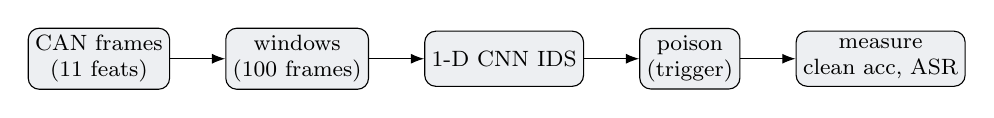
\begin{tikzpicture}[font=\footnotesize,>=Latex,node distance=4mm and 7mm,
  b/.style={draw,rounded corners,align=center,fill=accent!8,minimum height=7mm,inner sep=2.5pt}]
\node[b](a){CAN frames\\(11 feats)};
\node[b,right=of a](w){windows\\(100 frames)};
\node[b,right=of w](c){1-D CNN IDS};
\node[b,right=of c](p){poison\\(trigger)};
\node[b,right=of p](m){measure\\clean acc, ASR};
\draw[->](a)--(w);\draw[->](w)--(c);\draw[->](c)--(p);\draw[->](p)--(m);
\end{tikzpicture}
\caption{Preliminary attack pipeline (privacy defences added in IA-2).}\label{fig:flow}
\end{figure}

% ===== 3 =====
\section{Dataset Identification and Preliminary Preparation}\label{sec:data}
\textbf{Source.} HCRL in-vehicle CAN intrusion captures (OTIDS family) via the
public Kaggle mirror \texttt{bikashkundu/can-hcrl-otids}: one normal capture and
three attack captures. \textbf{Format:} \texttt{TS, ID1, ID0, LEN, DLC0--7,
target}. \textbf{Suitability:} real, labelled vehicle-network traffic with a clear
normal/attack split -- exactly what a CAN-IDS needs, and the trigger can be a CAN
ID absent from the data. \textbf{Preparation:} each frame
$\to[\Delta t,\text{ID},\text{DLC},b_0\ldots b_7]$; windows of 100 frames (stride
50), labelled by capture class, with a time-contiguous split \emph{inside} each
capture to prevent window leakage; standardised on training statistics. Full
provenance (row counts, SHA-256 hashes, licence) is in \texttt{data/PROVENANCE.md}.

% ===== 4 =====
\section{Initial Implementation and Demonstration}\label{sec:impl}
Code is in \texttt{src/canids/} (mechanisms from scratch; Opacus only for the
DP-SGD accountant); pipeline correctness is checked in \texttt{tests/}
(9 passing tests). The complete codebase is at
\url{https://github.com/aish475/MLCS_IA}.

\subsection{Honest detector}
Table~\ref{tab:det} shows the baseline IDS detects CAN intrusions almost perfectly
(CNN $F_1=\CNNfone$). A near-perfect detector is the right starting point: the
project's claim is that even this can be silently backdoored.
\begin{table}[htbp]\centering\caption{Honest intrusion detectors (preliminary).}\label{tab:det}
\begin{tabular}{lrrrrr}
\toprule
Detector & Acc. & Bal.\ acc. & Prec. & Recall & $F_1$ \\
\midrule
RandomForest & 0.946 & 0.948 & 1.000 & 0.897 & 0.946 \\
1D-CNN & 0.996 & 0.996 & 0.992 & 1.000 & 0.996 \\
\bottomrule
\end{tabular}
\end{table}

\subsection{First backdoor demonstration}
Table~\ref{tab:bd} and Figure~\ref{fig:bd} give the first poison sweep: the honest
model ignores the trigger (ASR $\approx\HonestASR$), but once a small fraction of
attack windows are poisoned, the trigger flips genuine attacks to ``Normal'' at a
high rate while clean accuracy stays near the honest baseline.
\begin{minipage}{0.5\textwidth}\centering
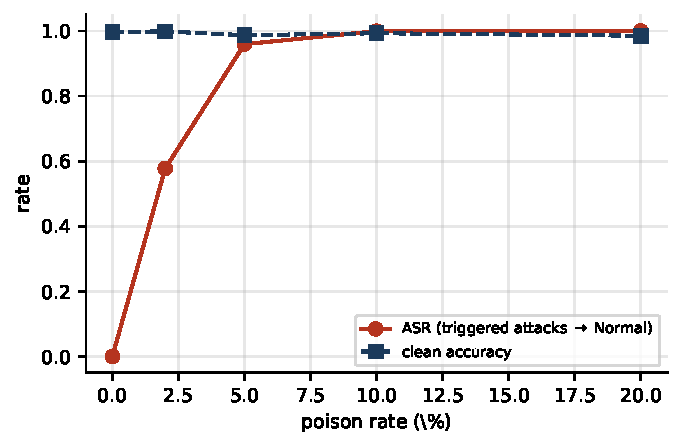
\includegraphics[width=\linewidth]{figs/backdoor.pdf}
\captionof{figure}{Clean accuracy and ASR vs poison rate.}\label{fig:bd}\end{minipage}\hfill
\begin{minipage}{0.46\textwidth}\centering
\captionof{table}{Backdoor poison sweep (preliminary).}\label{tab:bd}
\begin{tabular}{lrr}
\toprule
Poison rate & Clean acc. & ASR \\
\midrule
0\% & 0.997 & 0.000 \\
2\% & 0.999 & 0.578 \\
5\% & 0.987 & 0.959 \\
10\% & 0.993 & 0.999 \\
20\% & 0.985 & 1.000 \\
\bottomrule
\end{tabular}
\end{minipage}

% ===== 5 =====
\section{Preliminary Evaluation and Documentation}\label{sec:eval}
\subsection{Observations}
\begin{itemize}
\item The honest CNN is an almost perfect detector, so any successful backdoor is,
by construction, invisible on clean traffic.
\item The trigger causally affects only the poisoned model -- the honest model's
response to the trigger is near zero -- which isolates the attack from ordinary
misclassification.
\end{itemize}

\subsection{Evaluation plan for IA-2}
Detection: accuracy, balanced accuracy, attack precision/recall/$F_1$. Backdoor:
ASR, clean-accuracy gap, poison-rate sweep. Privacy: $\varepsilon$ (at
$\delta=10^{-5}$), ASR-vs-$\varepsilon$ and membership-inference AUC under DP-SGD;
LDP estimator utility vs local budget; compressive $F_1$ vs dimension. All over
multiple seeds.

\subsection{Individual-contribution statement}
\begin{shaded}\small\noindent I, \textbf{Aishwarya Nitin Gawali} (16014223007, B1),
designed the backdoored-CAN-IDS study and wrote the \texttt{src/canids} package
from scratch -- the HCRL parser and time-contiguous windowing, the 1-D CNN
(GroupNorm, DP-SGD-ready) and RandomForest detectors, the trigger-injection and
poisoning code with the ASR measurement, and the scaffolding for the local-DP,
compressive and membership-inference components completed in IA-2 -- together with
the unit tests and the experiment driver. Opacus is used only as the DP-SGD
accountant.\end{shaded}

\bibliographystyle{plainnat}
\bibliography{refs}
\end{document}
